%----------------------------------------------------------------------------
%
%	This template was created by
%		Christian Krieg <christian.krieg@alumni.tuwien.ac.at>
%
%	April 2018
%
%----------------------------------------------------------------------------
%
\documentclass[%
	a4paper,
]
{article}
%
%----------------------------------------------------------------------------
%
% Institution
%
%\institution{Institute of Computer Technology}

%
%----------------------------------------------------------------------------
%
% Use the 'Libertine' font type
%
\usepackage{libertine}
\usepackage[T1]{fontenc}
\usepackage[utf8]{inputenc}
%
%----------------------------------------------------------------------------
%
% Set page margins
%
\usepackage{geometry}
\geometry{%
	left   = 2cm,
	right  = 2cm,
	top    = 2cm,
	bottom = 2cm
}
%
%----------------------------------------------------------------------------
%
% Set line spacing
%
\usepackage{setspace}
\setstretch{1.2}
%
%----------------------------------------------------------------------------
%
% Set paragraph: No indentation, but include an empty line
%
\usepackage[parfill]{parskip}
%
%----------------------------------------------------------------------------
%
% Set justification in algorithms
%
\usepackage{ragged2e}
%
%----------------------------------------------------------------------------
%
% Use colors
%
\usepackage{xcolor}
\usepackage{colortbl}
%
%----------------------------------------------------------------------------
%
% Define a TODO and a DONE command
%
\newcommand{\todo}[1]{\textcolor{red}{#1}}
\newcommand{\done}[1]{}
%
%----------------------------------------------------------------------------
%
% Use glossaries
%
\usepackage{glossaries}
%
% Glossary entries
%
\makenoidxglossaries

\newglossaryentry{oc}{
	name = {OpenCores},
	description = { A wegpage (opencores.org), which provides open source Hardware Design Language Intellectual Properties },
	text = {OpenCores},
	first = { OpenCores },
	plural = {FPGAs},
	firstplural = {field-programmable gate arrays (FPGAs)},
}
%
\newglossaryentry{url}{
	name = {URL},
	description = { A name used to address a ressource located on a computer or in a computer network },
	text = {URL},
	first = { Uniform Ressource Locator (URL)},
	plural = {URLs},
	firstplural = {Uniform Ressource Locators (URLs)},
}
%
\newglossaryentry{python}{
  name={Python},
  description={ A interpretive programming language },
  text={Python},
  first={ Python },
}
%
\newglossaryentry{hdl}{
  name={HDL},
  description={Hardware description language; A language to describe the function of Digital Hardware textually.},
  text={HDL},
  first={hardware description language (HDL)},
  plural={HDLs},
  firstplural={hardware description languages (HDLs)},
}
%
\newglossaryentry{vhdl}{
  name={VHDL},
  description={Very-high-speed integrated circuits hardware description language. See also \gls{hdl}},
  text={VHDL},
  first={very-high-speed integrated circuits hardware description
		language (VHDL)},
}
%
\newglossaryentry{rtl}{
  name={RTL},
  description={Register-transfer level; An abstraction layer of digital hardware designs, where the function is described with logical gates, like an AND-Gate},
  text={RTL},
  first={register-transfer level (RTL)},
}

\newglossaryentry{scraper}{
 name={Scraper},
 description={ A piece of software, that transforms information optimised for human readability into machine oriented data sets. },
 text={Scraper},
 first={Scraper},
 plural={Scrapers},
 firstplural={Scraper},
}

\newglossaryentry{IP}{
 name={IP},
 description={Intellectual Property; Non-Physical products, which may be protected by a copyright. In the context of this document, IP refers to a Hardware Design.},
 text={IP},
 first={Intellectual Property (IP)},
 plural={IPs},
 firstplural={Intellectual Properties (IPs)},
}

\newglossaryentry{scrapy}{
 name={Scrapy},
 description={A Web Scraper based on Python. See also \gls{scraper}},
 text={Scrapy}
}

\newglossaryentry{html}{
  name={HTML},
  description={Hyper Text Markup Language; A language to describe the layout of text and media.},
  text={HTML},
  first={Hyper Text Markup Language (HTML)},
}

\newglossaryentry{hyperlink}{
  name={hyperlink},
  description={Points to another location/ressource on the internet},
  text={Hyperlink},
  plural={Hyperlinks},
}

%
%\newglossaryentry{}{
%  name={},
%  description={},
%  text={},
%  first={},
%  plural={},
%  firstplural={},
%}
%----------------------------------------------------------------------------
%
% Settings for citations and the bibliography
%
\usepackage[%
	backend     = biber,
	maxbibnames = 99,
	citestyle   = numeric,
	autocite    = plain,
%	autocite    = footnote,
%	citestyle   = verbose-ibid,
	giveninits=true,
]{biblatex}
\bibliography{bib/bakk}
%
%----------------------------------------------------------------------------
%
% For Pseudo code
%
\usepackage[ruled]{algorithm2e}
\renewcommand{\algorithmcfname}{ALGORITHM}
\SetAlFnt{\normalsize}
\SetAlCapFnt{\normalsize}
\SetAlCapNameFnt{\normalsize}
%\SetAlCapHSkip{0pt}
%\IncMargin{-\parindent}
%
%----------------------------------------------------------------------------
%
%	TikZ -- TikZ ist kein Zeichenprogramm
%

 \usepackage{tikz}
% \usepackage{tikz-timing}
% \usepackage{etoolbox}
% \usetikzlibrary{mindmap}
% \usetikzlibrary{shapes}
% \usetikzlibrary{arrows}
% \usetikzlibrary{decorations}
% \usetikzlibrary{shapes.symbols}
% \usetikzlibrary{shapes.geometric}
% \usetikzlibrary{shapes.multipart}
% \usetikzlibrary{positioning}
% \usetikzlibrary{patterns}
% \usetikzlibrary{calc}
% \usetikzlibrary{scopes}         % cf. pgfmanual p.66
% \usetikzlibrary{chains}         % cf. pgfmanual p.284
% \usetikzlibrary{fit}
% \usetikzlibrary{matrix}
% \usetikzlibrary{decorations}
% \usetikzlibrary{circuits.logic}
% \usetikzlibrary{circuits.logic.IEC}
% \usetikzlibrary{shapes.gates.logic.IEC}
% %\usetikzlibrary{circuits.logic.US}
% %\usetikzlibrary{shapes.gates.logic.US}
% \usetikzlibrary{circuits.ee}
% \usetikzlibrary{circuits.ee.IEC}
% \usetikzlibrary{backgrounds}
% \usetikzlibrary{automata}
% \usetikzlibrary{intersections}
% \usetikzlibrary{plotmarks}
% \usepgflibrary{fpu}
% \usetikzlibrary{decorations.pathreplacing}
%
%----------------------------------------------------------------------------
%
% TikZ shapes
%  
    \usepackage{pgfplots,siunitx}
    \pgfplotsset{compat=1.16}
    \usepackage{graphicx}
	\graphicspath{{fig/}}
	\usepackage[section]{placeins}
%
%----------------------------------------------------------------------------
%
% Use AMS math fonts
%
\usepackage{amsfonts}
\usepackage[sans]{dsfont}
%
%----------------------------------------------------------------------------
%
% Use multiple figures in one float
%
\usepackage{subcaption}
%
%----------------------------------------------------------------------------
%
% Use dummy text
%
\usepackage{lipsum}
%
%----------------------------------------------------------------------------
%
% Use extended list environments (e.g., 'inparaenum')
%
\usepackage{paralist}
%
%----------------------------------------------------------------------------
%
% Define Colours
%
\definecolor{mygreen}{rgb}{0,0.6,0}
\definecolor{mygray}{rgb}{0.5,0.5,0.5}
\definecolor{mymauve}{rgb}{0.58,0,0.82}
%
%----------------------------------------------------------------------------
% Use listings
%
\usepackage{listings}

\lstdefinestyle{vhdl}
{
	language=VHDL,
  basicstyle=\linespread{1}\scriptsize\ttfamily\color{black},
  commentstyle=\scriptsize\itshape,
  escapeinside={(*@}{@*)},
  frame=single, numbers=left,
%  numbersep=5pt,
  xleftmargin=15pt,
  xrightmargin=5pt,
  numbersep=5pt,
  breaklines=true,
  moredelim=**[is][\ttfamily\bfseries\color{red}]{(*}{*)},
}

\lstdefinestyle{verilog}
{
	language=Verilog,
  basicstyle=\linespread{1}\scriptsize\ttfamily\color{black},
  commentstyle=\scriptsize\itshape,
  escapeinside={(*@}{@*)},
  frame=single, numbers=left,
%  numbersep=5pt,
  xleftmargin=15pt,
  xrightmargin=5pt,
  numbersep=5pt,
  breaklines=true,
  moredelim=**[is][\ttfamily\bfseries\color{red}]{(*}{*)},
}

\lstdefinestyle{python}
{
  language=python,
  backgroundcolor=\color{white},   % choose the background color; you must add \usepackage{color} or \usepackage{xcolor}; should come as last argument
  basicstyle=\footnotesize,        % the size of the fonts that are used for the code
  breakatwhitespace=false,         % sets if automatic breaks should only happen at whitespace
  breaklines=true,                 % sets automatic line breaking
  captionpos=b,                    % sets the caption-position to bottom
  commentstyle=\color{mygreen},    % comment style
  deletekeywords={...},            % if you want to delete keywords from the given language
  escapeinside={\%*}{*)},          % if you want to add LaTeX within your code
  extendedchars=true,              % lets you use non-ASCII characters; for 8-bits encodings only, does not work with UTF-8
  frame=single,	                   % adds a frame around the code
  keepspaces=true,                 % keeps spaces in text, useful for keeping indentation of code (possibly needs columns=flexible)
  keywordstyle=\color{blue},       % keyword style
  morekeywords={*,...},            % if you want to add more keywords to the set
  numbers=left,                    % where to put the line-numbers; possible values are (none, left, right)
  numbersep=5pt,                   % how far the line-numbers are from the code
  numberstyle=\tiny\color{mygray}, % the style that is used for the line-numbers
  rulecolor=\color{black},         % if not set, the frame-color may be changed on line-breaks within not-black text (e.g. comments (green here))
  showspaces=false,                % show spaces everywhere adding particular underscores; it overrides 'showstringspaces'
  showstringspaces=false,          % underline spaces within strings only
  showtabs=false,                  % show tabs within strings adding particular underscores
  stringstyle=\color{mymauve},     % string literal style
}
%
%----------------------------------------------------------------------------
%
% Typeset pseudo code
%
\usepackage{syntax}
\usepackage{amssymb}
%----------------------------------------------------------------------------
%
% More options for boxes
%
\usepackage{realboxes}
%
% Command for vertical text in tabulars
%
\newcommand*\rot{\rotatebox{90}}
%
%----------------------------------------------------------------------------
%
\usepackage{makecell}
%
%----------------------------------------------------------------------------
%
% Package for logos (e.g., the BibTeX logo)
%
\usepackage{dtk-logos}
%
%----------------------------------------------------------------------------
%
% Use \textsubscript
%
%\usepackage{fixltx2e}
%
%----------------------------------------------------------------------------
%
% More options for tabulars
%
\usepackage{array}
\usepackage{tablefootnote}
\usepackage{threeparttable}
%
%----------------------------------------------------------------------------
%
% Support long tables
%
\usepackage{longtable}
%
%----------------------------------------------------------------------------
%
% Use appendices
%
\usepackage[titletoc]{appendix}
%
%----------------------------------------------------------------------------
%
% Settings for hyperlinks
%
\usepackage{hyperref}
\hypersetup{%
	colorlinks = true,
	allcolors  = blue,
}
%

%
%----------------------------------------------------------------------------
%
% Use the cleverref package -- Load this package as the very last!
%
\usepackage{cleveref}
%
%----------------------------------------------------------------------------
%
% Document body
%
\begin{document}
%
%----------------------------------------------------------------------------
\begin{titlepage}

	\begin{center}

	
\includegraphics[height=2cm]{fig/logo-tu-bw.png}%
	\hfill{}%
	
\includegraphics[height=2cm]{fig/logo-ict.png}%
	

	\vspace{5em}


		\large
		David FREISMUTH\\
	

	\vspace{5em}

		{\huge Bachelor Thesis}\\[1em]
		{\Large 384.088, Winter Term 2018} \\[2em]
		{\large Supervisor:\\[.5em]
			DI Christian Krieg} \\[5em]

		\today
		\vspace{5em}

		{\Huge Development of a testing environment for an automatic Hardware Design Classification }\\[2em]

		\vspace{3em}
	\end{center}

\end{titlepage}
%
%----------------------------------------------------------------------------
%
%\vspace*{27em}

Copyright (C) 2018 Christian Krieg, David Freismuth

If you find this work useful, please cite it using the following \BibTeX{ } entry:

\vspace{1em}


\vspace{3em}
Contact us:

\href{christian.krieg@alumni.tuwien.ac.at}{christian.krieg@alumni.tuwien.ac.at}

\vfill


\includegraphics[height=1.5cm]{fig/cc-large.png}

\includegraphics[height=1.5cm]{fig/by-large.png}


This documentation is licensed under the following license:
Attribution 4.0 International (CC BY 4.0)

\vspace{3em}

You are free to:

\begin{enumerate}
    \item Share --- Copy and redistribute the material in any medium or format
    \item Adapt --- Remix, transform, and build upon the material for any purpose,
			even commercially.
\end{enumerate}

This license is acceptable for Free Cultural Works.

The licensor cannot revoke these freedoms as long as you follow the license terms.

The entire license text is available at:
\href{https://creativecommons.org/licenses/by/4.0/legalcode}
	{https://creativecommons.org/licenses/by/4.0/legalcode}


\pagebreak
%
%----------------------------------------------------------------------------
%
\newgeometry{%
	left   = 3.5cm,
	right  = 3.5cm,
	top    = 2cm,
	bottom = 2cm
}

%%%%%%%%%%%%%%%%%%%%%%%%%%%%%%%%%%%%%%%%%%%%%%%%%%%%%%%%%%%%%%%%%%%%%%%%%%%%%%%%
%                                                                              %
%	File:     abstract.tex                                                     %
%   Document: XXX	                                                           %
%   Author:   Freismuth David                                                  %
%	Date:	  22.JUN.2018                                                      %
%   Content:  Contains the abstract section of the Bachelor thesis.            %
%                                                                              %
%%%%%%%%%%%%%%%%%%%%%%%%%%%%%%%%%%%%%%%%%%%%%%%%%%%%%%%%%%%%%%%%%%%%%%%%%%%%%%%%

%%%%%%%%%%%%%%%%%%%%%%%%%%%%%%%%%%%%%%%%%%%%%%%%%%%%%%%%%%%%%%%%%%%%%%%%%%%%%%%%
\paragraph{Abstract}
Due to increasing size and complexity of modern hardware designs, the challenge
of identifying a piece of design becomes increasingly difficult. This is especially
true, if no documentation is available. This factor has a direct impact on the 
time that is needed to get familiar with a design. In extreme cases, the design
is rendered useless for the user. A hint on what hardware category the design 
belongs to, would accelerate the process of familiarization.
This work considers, if it is possible to categorize hardware designs, that are
given as Hardware Description Language, on basis of their structure. 
The elaborated algorithm is able to categorize a given design in X seconds, with
an accuracy of S.

%%%%%%%%%%%%%%%%%%%%%%%%%%%%%%%%%%%%%%%%%%%%%%%%%%%%%%%%%%%%%%%%%%%%%%%%%%%%%%%%
\paragraph{Kurzfassung}
Mit steigender Größe und Komplexität von modernen Hardware Designs, wird es 
zusehends herausfordernder die Funktion des desselben zu identifizieren. Vor
allem trifft dies zu, wenn keine Dokumentationen zum Design verfügbar sind. Dieser 
Umstand wirkt sich unmittelbar in einer erhöhten Einarbeitungszeit aus. In Extremfällen 
muss der Anwender das Design wegen Unbrauchbarkeit verwerfen. Ein Hinweis darauf welcher
Hardware Kategorie das Design angehört, würde den Einarbeitungsprozess beschleunigen.
Diese Arbeit untersucht, ob es möglich ist Hardware Designs, die als Hardware
Description Language vorliegen, anhand ihres strukturellen Aufbaus zu klassifiziern, 
und in Kategorien einzuteilen. 
Mithilfe des erarbeiteten Algorithmus ist es möglich ein Design innerhalb von X 
Sekunden, mit einer Sicherheit von Y zu klassifiziern. 

\tableofcontents
\clearpage
\printnoidxglossaries
%%%%%%%%%%%%%%%%%%%%%%%%%%%%%%%%%%%%%%%%%%%%%%%%%%%%%%%%%%%%%%%%%%%%%%%%%%%%%%%%
%                                                                              %
%	File:     introduction.tex                                                 %
%   Document: XXX	                                                           %
%   Author:   Freismuth David                                                  %
%	Date:	  22.JUN.2018                                                      %
%   Content:  Contains the Introduction section of the Bachelor thesis.        %
%                                                                              %
%%%%%%%%%%%%%%%%%%%%%%%%%%%%%%%%%%%%%%%%%%%%%%%%%%%%%%%%%%%%%%%%%%%%%%%%%%%%%%%%

%%%%%%%%%%%%%%%%%%%%%%%%%%%%%%%%%%%%%%%%%%%%%%%%%%%%%%%%%%%%%%%%%%%%%%%%%%%%%%%%
\section{Introduction}
As Embedded Systems find their way in an increasingly wide field of applications,
with growing demands to performance and relieability, the underlying Hardware 
Designs also gain in diversity, complexity and size. Since it is nearly impossible,
even for simple Designs, to determine the function of such, without proper
documentation, a possibility to extract information directly from the Hardware 
Description Language representation of the Design, seems to be a welcome aid.
Such a hardware design classification algorithm also allow services, which 
automatically handle aforementionend designs (for instance online sharing 
plattforms like gls{oc}) to assign categories without relying on user input.

\begin{figure}[h]
 \centering
 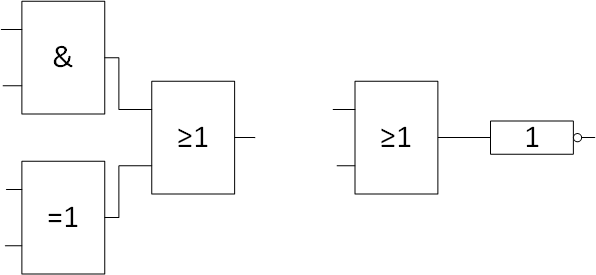
\includegraphics[width=\textwidth,keepaspectratio]{fig/logicGates.png}
 \caption{Example of a Two to One Connection (left) and an One to One Connection (right).}
 \label{fig:logicGates}
\end{figure}

This work tries to achieve a classification of hardware designs by analyzing the 
connection between logical cells. The count of specified two to one and one to 
one connections (examples depictioned in illustration), are translated into a
standardized match vector. It is expected that the match vector of similar designs
gather in clusters. These clusters can then be understood as hardware categories. 
Using a methodolodgy like this implies, that the location and meaning of those clusters first 
have to be identified, by analyzing a great amount of well known hardware designs.
The clustering is also in scope of this work, and is achieved by a web crawler,
which gathers already categorized designs from the open source sharing plattform 
gls{oc}. These designs are then synthesized by the open source synthesis tool 
gls{yosys} and handed over to the match algorithm, which eventually determines 
the match vector. The so gathered set of match vectors are then grouped into clusters.

The result of this work is a <command line application> which is able to 
categorize large designs (XXX Cells) in X seconds with a certainty of Y%.
The following chapters elaborate on the development, set of problems and 
other possible applications of this work. 
  

%%%%%%%%%%%%%%%%%%%%%%%%%%%%%%%%%%%%%%%%%%%%%%%%%%%%%%%%%%%%%%%%%%%%%%%%%%%%%%%%
%                                                                              %
%	File:     sota.tex                                                         %
%   Document: XXX                                                              %
%   Author:   Freismuth David                                                  %
%	Date:	  22.JUN.2018                                                      %
%   Content:  Contains the State of the Art section of the Bachelor thesis.    %
%                                                                              %
%%%%%%%%%%%%%%%%%%%%%%%%%%%%%%%%%%%%%%%%%%%%%%%%%%%%%%%%%%%%%%%%%%%%%%%%%%%%%%%%

%%%%%%%%%%%%%%%%%%%%%%%%%%%%%%%%%%%%%%%%%%%%%%%%%%%%%%%%%%%%%%%%%%%%%%%%%%%%%%%%
\section{State of the Art}
Literature regarding this topic is very scarce, if not non-existent. At the timethis work has been released, no other publications, which attempted to establish 
an algorithm to automatically identify hardware designs, could be found.
Papers which worked on topics remotely relatable with the topic of hardware 
categorization, mostly presented methods to identify hardware trojans in a given 
design. This Hardware Trojan Identification can be seen as categorization into 
two groups: Non Hardware Trojan injected, and Hardware Trojan injected.
Identification of those Trojans is mostly achieved via a functional analysis [put sources here], where the design is simulated and tested for a certain
behaviour. Since our method aims for a structural analysis, these publications 
are hardly compareable to ours. Though one publication used a combination of structural- and 
functional analysis, to identify hardware trojan design patterns. This 
methodolodogy should be further looked upon.  

\subsection{Detection of Hardware Trojans}
In \autocite{Oya2015} X net types are defined, which are typical for hardware trojans.
\label{hwTrojanNets} shows those proposed Hardware Trojans nets. Similar to 
our proposed method, the count of these nets are determined. 
 
\begin{figure}[h]
    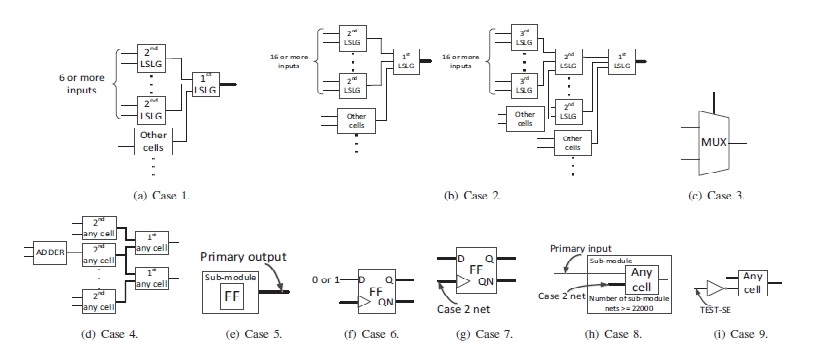
\includegraphics[width=\textwidth,keepaspectratio]{fig/hwTrojanNets.jpg}
    \label{hwTrojansNets}
    \caption{Register Transfer Level depiction of the proposed Hardware Trojan nets \autocite{Oya2015}}
\end{figure}

The publication states, that trough the count of certain net types, the presence
of hardware trojans can be determined, but not their absence.
This insight leads to the assumption, that hardware design can be classified 
using the count of certain net types. 

%%%%%%%%%%%%%%%%%%%%%%%%%%%%%%%%%%%%%%%%%%%%%%%%%%%%%%%%%%%%%%%%%%%%%%%%%%%%%%%%
%                                                                              %
%   File:     metholodgy.tex                                                   %
%   Document: XXX	                                                           %
%   Author:   Freismuth David                                                  %
%	Date:	  22.JUN.2018                                                      %
%   Content:  Contains the Metholodgy section of the Bachelor thesis.          %
%                                                                              %
%%%%%%%%%%%%%%%%%%%%%%%%%%%%%%%%%%%%%%%%%%%%%%%%%%%%%%%%%%%%%%%%%%%%%%%%%%%%%%%%

%%%%%%%%%%%%%%%%%%%%%%%%%%%%%%%%%%%%%%%%%%%%%%%%%%%%%%%%%%%%%%%%%%%%%%%%%%%%%%%%
\section{Methodology}

To achieve our goal of the categorization of hardware designs trough a structural analysis of the corresponding HDL Design, we firstly propose a non-standardized match vector, which contains the count of the Design's Two-to-One and One-to-One Gate Level Connections (see \label{logicGates} referencce) as each of its entries, and secondly a standardized match vector, which reduces the information hold by the non-standardized match vector down to a two dimensional vector. This standardized match vector shall then act as categorization criteria, to sort the design into predefined design categories. Those categories are clusters in the vector space the standardized match vector is part of. If the match vector points into such a cluster, the design is identified with the corresponding category.
This section elaborates on the details of finding a match vector of a design, and
how the category clusters are defined. 

\subsection{Cluster Identification}
As mentionend above, before any categorization can take place, the categories itself
have to be defined. In our model, categories are clusters in a two dimensional vector space. 
Therefore, the task is to identify clusters in this vector space, and name them. 
To do this, we determine the match vectors of well known designs. Since
the categorization of those designs is already available, the vectors that originate from designs with identical categorizations, can be grouped together to clusters. 

It is expected, that the validity of such clusters increases with the number of analyzed designs. Therefore an automatic process has to be established, to enable the analysis of a great amount of designs. Conveniently, the website \gls{oc} offers a great collection of Hardware Designs that already have been categorised manually. \gls{oc} though does not offer an interface to automatically download all available design files. Therefore it has to be resorted to the web page, which is optimized for human interaction, but not for machine readability. Luckily there are Tools, which are spezialized in translating human readable content into structured, machine oriented data sets. These are called \glspl{scraper}. \gls{scrapy} \autocite{scrapy} is a python framework that exposes the functionallities of such a \gls{scraper}, and provides multiple python classes which enable extensible web scraping. Because of its ease of use and extensibility, \gls{scrapy} has been chosen, to solve the majority of problems that come with the challenge of retrieving a great amount of Hardware Designs.

Among the set of information that is specifically provided for each design by \gls{oc}, we fetch and process following information.  

\begin{enumerate}

	\item{\gls{url} to the design archive}
       
       So the Cluster Identification can be validated at a later point in time (asuming the files still exist under the same link).

	\item{The name of the design project}
       
       Used to address single designs. 

	\item{The \gls{hdl} in which the design is specified and implemented}
       
       Necesarry for the synthesis process, later in the cluster identification process

	\item{The category in which a design is listed}
       
       Mandatory for the Cluster identification process. 
        
	\item{The \gls{hdl} files of the design}
       
       Trivially necesarry to analyse the hardware design.
        
\end{enumerate}

Scrapy is able to process data within a pipeline structure, which, in our case, enables us to push user defined data sets trough those stages, an perform specific actions on them. The advantage herein lies in the parallelity, and therefore speed increase, that can be achieved by using this strucutre, since multiple pipelines can be active at a given time. \cref{fig:scrapyPipeline} shows the pipeline stages of the scrapy implementation that has been developed during the run of this thesis.
The following chapters explain in detail, how those Pipeline stages manipulate the data stated in the enumeration above.

\begin{figure}
    \centering
    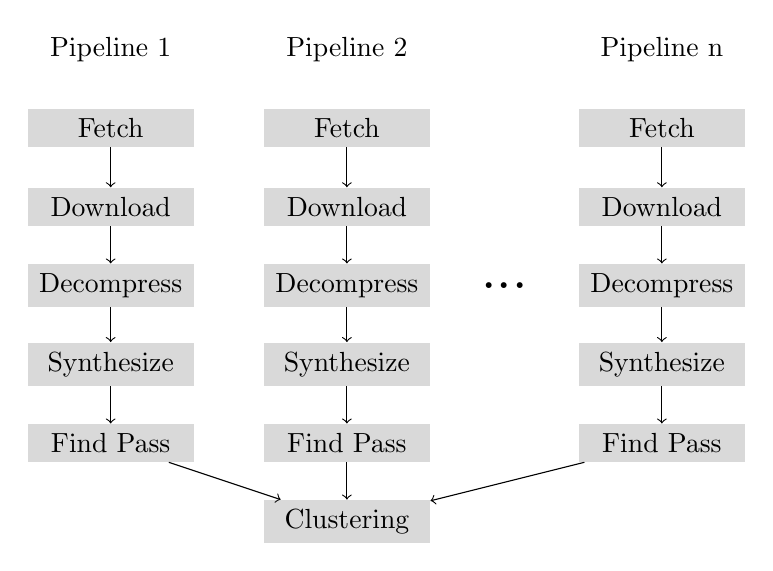
\begin{tikzpicture}[scale = 1]
        \tikzstyle{every node} = [scale = 1, rectangle, fill=gray!30, minimum width = 6em, minimum height = 1em)]
        \node(Pipeline 1)[fill = white] at (0, 0) {Pipeline 1};
        \node(Fetch1) at (0, -1){Fetch};
        \node(Download1) at (0, -2) {Download};
        \node(Decompress1) at (0, -3) {Decompress};
        \node(Synthesize1) at (0, -4) {Synthesize};
        \node(Find pass1) at (0, -5) {Find Pass};
        \draw [->] (Fetch1) -- (Download1);
        \draw [->] (Download1) -- (Decompress1);
        \draw [->] (Decompress1) -- (Synthesize1);
        \draw [->] (Synthesize1) -- (Find pass1);
        
        \node(Pipeline 2)[fill = white] at (3, 0) {Pipeline 2};
        \node(Fetch2) at (3, -1){Fetch};
        \node(Download2) at (3, -2) {Download};
        \node(Decompress2) at (3, -3) {Decompress};
        \node(Synthesize2) at (3, -4) {Synthesize};
        \node(Find pass2) at (3, -5) {Find Pass};
        \draw [->] (Fetch2) -- (Download2);
        \draw [->] (Download2) -- (Decompress2);
        \draw [->] (Decompress2) -- (Synthesize2);
        \draw [->] (Synthesize2) -- (Find pass2);
        
        \node(ellipsis)[fill = none, scale = 2] at (5,-3) {...};
        
        \node(Pipeline n)[fill = white] at (7, 0) {Pipeline n};
        \node(Fetchn) at (7, -1){Fetch};
        \node(Downloadn) at (7, -2) {Download};
        \node(Decompressn) at (7, -3) {Decompress};
        \node(Synthesizen) at (7, -4) {Synthesize};
        \node(Find passn) at (7, -5) {Find Pass};
        \draw [->] (Fetchn) -- (Downloadn);
        \draw [->] (Downloadn) -- (Decompressn);
        \draw [->] (Decompressn) -- (Synthesizen);
        \draw [->] (Synthesizen) -- (Find passn);
        
        \node(Clustering) at (3, -6) {Clustering};
        \draw [->] (Find pass1) -- (Clustering);
        \draw [->] (Find pass2) -- (Clustering);
        \draw [->] (Find passn) -- (Clustering);
        

    \end{tikzpicture}
    \label{fig:scrapyPipeline}   
    \caption{ Pipeline stages of the \gls{scrapy} implementaion. As seen in the figure, Pipelines can be executed parallelly. The final stage "Clustering" is not implemented as pipeline stage, but rather waits on the completion of all pipelines to process all the gathered data. }
\end{figure}

\subsubsection{Fetch} 
In this stage, the \gls{oc} site is called to find the \glspl{url} where the hardware designs and corresponding meta informaiton resides. As \gls{oc}'s web page is built, like most web pages, in a tree like structure (see \cref{fig:opencoresStructure} for reference), \gls{scrapy} has been configured to start from the root page www.opencores.org, where the links to all projects reside (corresponds to the function call in \cref{lst:scrapyMainClass} line >>XXXX<<). "Start" in this context means, that the \Gls{html} representation of the site is retrieved by \gls{scrapy} and exposed via a \Gls{python} class to the User. \Gls{scrapy} then offers functions to extract informations from the \gls{html} code, like filtering for all <h> elements (which represent \glspl{hyperlink} that fork deeper into the website.).

\begin{figure}
 \centering
 \begin{tikzpicture}[grow via three points={one child at (0.5,-0.7) and two children at (0.5,-0.7) and (0.5,-1.4)},
  edge from parent path={(\tikzparentnode.south) |- (\tikzchildnode.west)}]
  \tikzstyle{every node}=[draw=black,thick,anchor=west]
  \tikzstyle{selected}=[draw=red,fill=red!30]
  \tikzstyle{optional}=[dashed,fill=gray!50]
  \node {opencores.org}
    child { node {opencores.org/projects}
        child{ node [selected] {opencores.org/project/audio}}
        child{ node [selected] {opencores.org/project/adder_subtractor}}
        child{ node [selected] {opencores.org/project/...}}
    }
    child [missing] {}
    child [missing] {}
    child [missing] {}
    child { node {opencores.org/forum}}
    child { node {opencores.org/licensing}}
    child { node {opencores.org/...}};
 \end{tikzpicture}
 \caption{The structure of the \gls{oc} website. The \Glspl{url} where the projects are located, are marked red.}
 \label{fig:opencoresStructure}
\end{figure}


As seen in \cref{lst:scrapyMainClass} line >>XXXXX<< for each >>element<<< that has been found, a new function >>>function<<< is invoked, which further calls the webpage the >>elements<< points to. 

\begin{lstlisting}[style = python, caption = {Scrapy Main Class}, label = {lst:scrapyMainClass}]
 class IPspider_oc(scrapy.Spider):
    """The class, which is called by the scrapy framework. """
    name = 'ipspider_oc'   # the name of the spider

    def start_requests(self):
        return [scrapy.Request(
          url = "https://opencores.org",
          callback=self.login)]

    def login(self, response):
        return scrapy.FormRequest.from_response( 
          response, 
          formdata={'user' : 'davFreismuth',  
                    'pass' : 'Qlghkeul'}, 
          callback=self.redirect )

    def redirect(self,  response):
        return scrapy.Request( 
          url = "https://opencores.org/projects?lang=0&stage=5&license=0&wishbone_version=0", 
          callback=self.parse )
                                                
    def parse(self, response):
        """Default callback for scrapy. Starts at start_url, fetches the url of the different project pages, and calls parse_metadata for each project page"""
        for href in response.css('td.project a::attr(href)'):
            yield response.follow(href, self.parse_metadata)

    def parse_metadata(self, response):
        """parses metadata of an opencore.org project page and returns a scrapy item object."""
        def scrape_line(strArray,  removeStr):  
            '''helper function which iterates trough the string array 'strArray', selects the first entry which contains 'removeStr' and returns the string without removeStr and whitespaces.'''
            for str in strArray:
                if(str.find(removeStr) != -1):
                    retStr = str.replace(removeStr,  '')
                    return retStr.strip()
            
        def scrape_href(line):  
            """helper function, which gets an html <a> element, checks if it has inner html and returns the text of the inner html"""
            start = line.find(">")
            end = line.find("<", start)
            if((start + 1) == end):
                return ""
            else:
                return line[(start+1):(end)]
            
        #fill up the fields
        hdl_IP =  HDL_IP()
        hdl_IP['name'] = scrape_line(response.css('h2 + p::text').extract(), 'Name:')
        hdl_IP['created'] = scrape_line(response.css('h2 + p::text').extract(), 'Created:')
        hdl_IP['updated'] = scrape_line(response.css('h2 + p::text').extract(), 'Updated:')
        hdl_IP['file_urls'] = ['https://opencores.org' + response.css('p a::attr(href)')[1].extract()]
        category = scrape_href(response.css('p a')[5].extract())
        category = category.lower()
        category = category.replace(' ', '_')
        hdl_IP['category'] = category
        hdl_IP['language'] = scrape_href(response.css('p a')[6].extract())
        hdl_IP['license'] = scrape_line(response.css('h2 + p::text').extract(),  'License:')
        hdl_IP['basePath'] = self.settings['FILES_STORE']
        yield hdl_IP
\end{lstlisting}

\paragraph*{Authentication \\}

Besides navigating to and trough the webpage, another task for the Fetch stage is the authentication with the \Gls{oc} user system, since designs are only downloadable, while logged in with a cost free \Gls{oc} account.

Login information is often communicated via \Gls{html} \Gls{post} Messages, which encode the message content into the message header. In the login case, the login information is encoded into the message header. After the login information has been accepted by the web page, it returns an authentication token, which is stored as \Gls{cookie} and enables access to the web page. Scrapy is natively able to generate and send such \Gls{post} messages and exposes the answer to such \Gls{post} messages in Python classes, for further actions. The function which sends the \Gls{post} message can be seen in \cref{lst:scrapyMainClass} line >>XXXXX<<.

\paragraph*{Extraction \\}
Once \Gls{scrapy} navigated to the project page, the above mentionend information is extracted by using \Gls{css} selectors, as seen in \cref{lst:scrapyMainClass} line >XXXXXX< to >>YYYYYYYY<<. The so gathered data sets are stored in the user defined \Gls{python} \lstinline{HDL_IP} object (derived from the \Gls{scrapy} class \lstinline{item}), which serves as container that gets pushed trough the Pipeline stages. The Fetch stage ends with returning the \lstinline{HDL_IP} object to the \Gls{scrapy} framework, where it gets handed over to the next Pipeline stage.  

\begin{figure}[h]
	\centering
	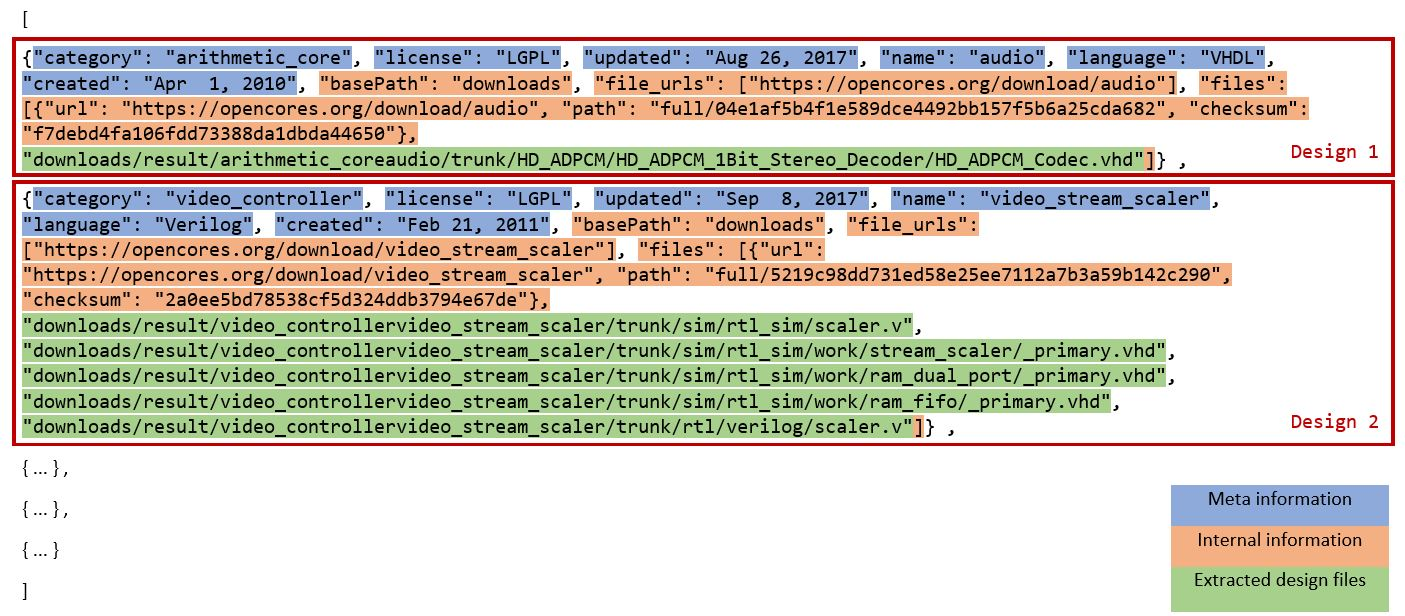
\includegraphics[width=\textwidth,keepaspectratio]{fig/jsonFileFormatDescription.JPG}
	\caption{.JSON File Format Description}
	\label{fig:jsonFormat}
\end{figure}

Figure \Cref{fig:jsonFormat} shows an example of the content of the .JSON file. 

\subsubsection{Download}
The \Gls{scrapy} \Gls{python} module provides the functionallity to automatically download and
store files that are associated with a Hardware design project, to a predefined
folder. The download is started by pushing an \lstinline{item} object with an \lstinline{URL} atrribute into a pipeline stage declared as a donwload stage. The \Gls{scrapy} framework then begins the download of the file specified in the \lstinline{URL} atrribute to the path defined in the atrribute \lstinline{spider.settings['FILE_STORE']}. If the file has been downloaded successfully, its name gets added to the \lstinline{HDL_IP} object under the attribute \lstinline{item.file}.  

\subsubsection{Decompress} 
Projects from \gls{oc} are solely provided eiter as *.tar.gz or *.zip compressed archive. The stage 'Decompress' is therefore dedicated to decompress the previously downloaded archive and to order the contained files into an predefined structure. The \Gls{python} modules \lstinline{tarfile} and \lstinline{zipfile} enable the extraction of such archives.
After the decompression, the project files are sorted into folders corresponding to 
their associated hardware category (as stated by \gls{oc}). After that, the file 
endings of the files are analysed. If those endings indicate a \gls{hdl} file, the path 
to this file is added to the aforementioned \lstinline{HDL_IP} object, in order to be able to
address the design files of a project in later stages. If no such files could be found, the \lstinline{HDL_IP} object is discarded, and will not be further processed. 

\subsubsection{Synthesis} 
After the design has been decompressed, it is time to let the synthesis tool \Gls{yosys} read the design files and synthesise them into a text file format. In order to do this in an automated manner, for each discovered design, a yosys script file is generated on the basis of the information, that has been gathered in previous steps. This Script instructs \Gls{yosys} about the path to the discovered files and with which frontend to load them. A sample script file can be seen in \cref{lst:yosysScriptFile}.
An alternative for this automatic script generation is to supply a custom made script, which will then be loaded instead of the generic one. Bigger design may need to be synthesised with such a custom script, since the dependecies may be much to complex, to be computed automatically. 

 \begin{lstlisting}[style = python, caption = {An example Yosys Script file.}, label = {lst:yosysScriptFile}]
  asdfsdafasdfasdfasdfsdaf
 \end{listing}
 \caption{An example Yosys Script file.}
 \label{lst:yosysScriptFile}
 \end{lstlisting}

The synthesis tool's frontend is chosen based on the language of each design file.
For \gls{vhdl} and SystemVerilog, the \lstinline{verific} frontend is used. For Verilog,
we use the \lstinline{read_verilog} frontend. Once any combination of \gls{hdl} files
has been loaded, a synthesize run attempts to generate a single HDL file from the provided
files, which solely contains primitive logic blocks. 

Since yosys does not support automatic dependency recognition of vhdl files, a custom solution
had to be found, to determine the load order of vhdl files (in the case that the user decides
that yosys scripts should be generated automatically). To accomplish this, we slightly modified 
the Vunit python project, which offers a function to return the \gls{vhdl} 
files in an ordered list. The vhdl files can then be loaded in the order dictated by this list.  

\subsubsection{Find Pass} 
Each design that is read by the synthesis tool is named after the project from
which the design files are downloaded. From then, the design name is the main
reference for each design and serves as identification feature in all
subsequent steps.

\subsubsection{Clustering}
blabla

\subsection{Design Identification}
blabla

\subsection{Verification}
blabla




%%%%%%%%%%%%%%%%%%%%%%%%%%%%%%%%%%%%%%%%%%%%%%%%%%%%%%%%%%%%%%%%%%%%%%%%%%%%%%%%
%                                                                              %
%	File:     conclusion.tex                                               %
%       Document: XXX	                                                       %
%       Author:   Freismuth David                                              %
%	Date:	  22.JUN.2018                                                  %
%       Content:  Contains the Conclusion section of the Bachelor thesis.      %
%                                                                              %
%%%%%%%%%%%%%%%%%%%%%%%%%%%%%%%%%%%%%%%%%%%%%%%%%%%%%%%%%%%%%%%%%%%%%%%%%%%%%%%%

%%%%%%%%%%%%%%%%%%%%%%%%%%%%%%%%%%%%%%%%%%%%%%%%%%%%%%%%%%%%%%%%%%%%%%%%%%%%%%%%
\section{Conclusion}
%%%%%%%%%%%%%%%%%%%%%%%%%%%%%%%%%%%%%%%%%%%%%%%%%%%%%%%%%%%%%%%%%%%%%%%%%%%%%%%%
%                                                                              %
%	File:     discussion.tex                                               %
%       Document: XXX	                                                       %
%       Author:   Freismuth David                                              %
%	Date:	  22.JUN.2018                                                  %
%       Content:  Contains the Discussion section of the Bachelor thesis.      %
%                                                                              %
%%%%%%%%%%%%%%%%%%%%%%%%%%%%%%%%%%%%%%%%%%%%%%%%%%%%%%%%%%%%%%%%%%%%%%%%%%%%%%%%

%%%%%%%%%%%%%%%%%%%%%%%%%%%%%%%%%%%%%%%%%%%%%%%%%%%%%%%%%%%%%%%%%%%%%%%%%%%%%%%%
\section{Discussion}

\printbibliography
\listoffigures

\end{document}
%
%----------------------------------------------------------------------------
